\chapter{Ten Puzzle Results}\label{chap:tenPuzzleSolving}

Figures~\ref{fig:firstSet10PuzzleInputImages} and~\ref{fig:secondSet10PuzzleInputImages} contain a set of 10~images of 5 different sizes that are made up of more than 5,800 total pieces.  These images were input into both the Mixed-Bag and Paikin~\& Tal solvers; this experiment represents twice as many puzzles as Paikin~\& Tal solved in~\cite{paikin2015}.

Figures~\ref{fig:firstSet10PuzzleMixedBagSolverImages} and~\ref{fig:secondSet10PuzzleMixedBagSolverImages} show the Mixed-Bag Solver outputs for this test set.  Four of the images (e.g., (a), (b), (e), (i)) are perfectly reconstructions.  The rest have only a small percentage of pieces out of place.  This is shown in the SEDAS visualizations in Figures~\ref{fig:firstSet10PuzzleMixedBagSedasImages} and~\ref{fig:secondSet10PuzzleMixedBagSedasImages}.  The Mixed-Bag Solver's output quality for these images is comparable to that of Paikin~\& Tal's algorithm when it solves these images individually.

\begin{figure}
\centering
  \begin{tabular}{ >{\centering\arraybackslash}m{0.45\textwidth} >{\centering\arraybackslash}m{0.45\textwidth} }

	\fbox{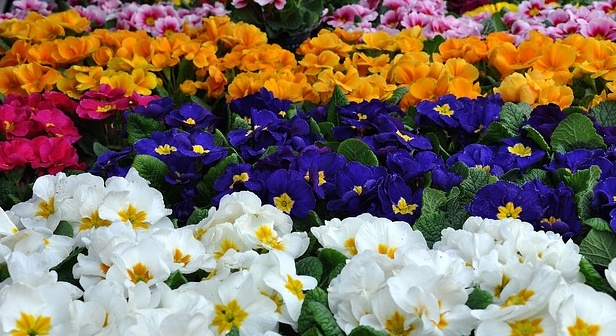
\includegraphics[scale=0.18]{./images/10_puzzles/primula_pixabay.jpg}} & \fbox{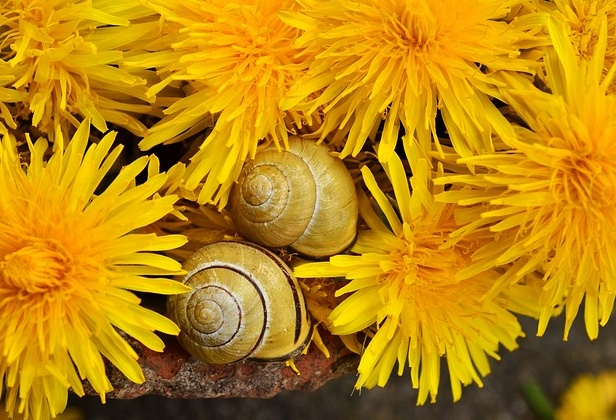
\includegraphics[scale=0.18]{./images/10_puzzles/dandelion_pixabay.jpg}} \\~\\
	Image~(a) \textendash { }264~pieces~\cite{pixabay} & Image~(b) \textendash { }330~pieces~\cite{pixabay}
\\~\\
	\fbox{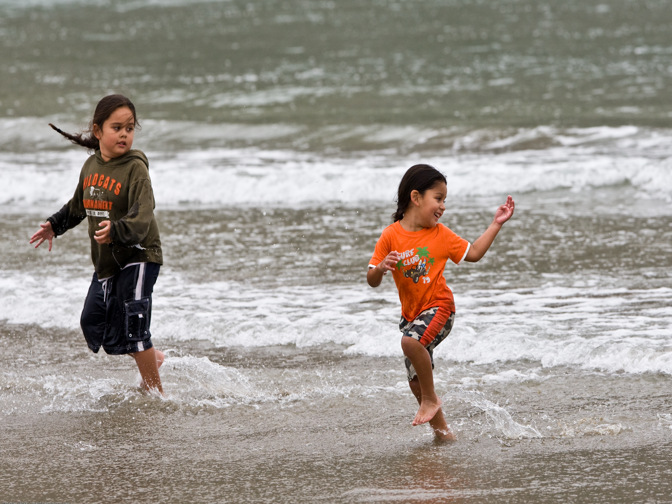
\includegraphics[scale=0.18]{./images/10_puzzles/cho_432_18.png}} & \fbox{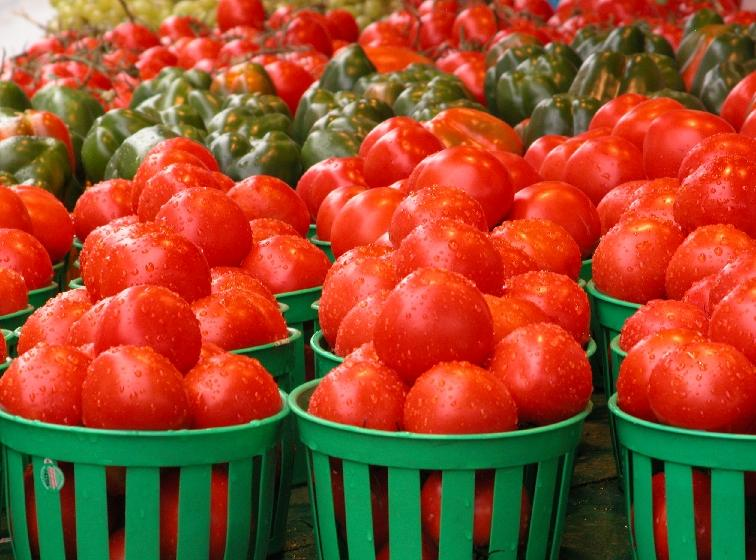
\includegraphics[scale=0.18]{./images/10_puzzles/mcgill_540_16.jpg}} \\~\\
	Image~(c) \textendash { }432~pieces~\cite{mcgillImageDatabase} & Image~(d) \textendash { }540~pieces~\cite{mcgillImageDatabase} 
\\~\\
	\fbox{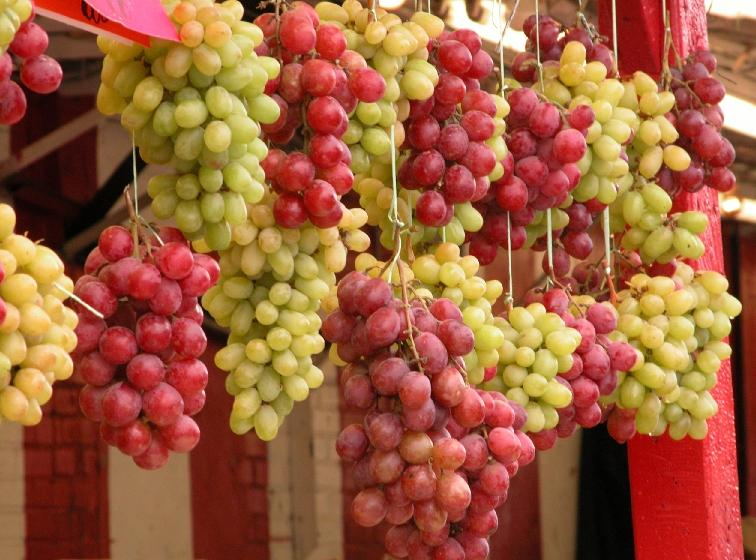
\includegraphics[scale=0.18]{./images/10_puzzles/mcgill_540_15.jpg}} & \fbox{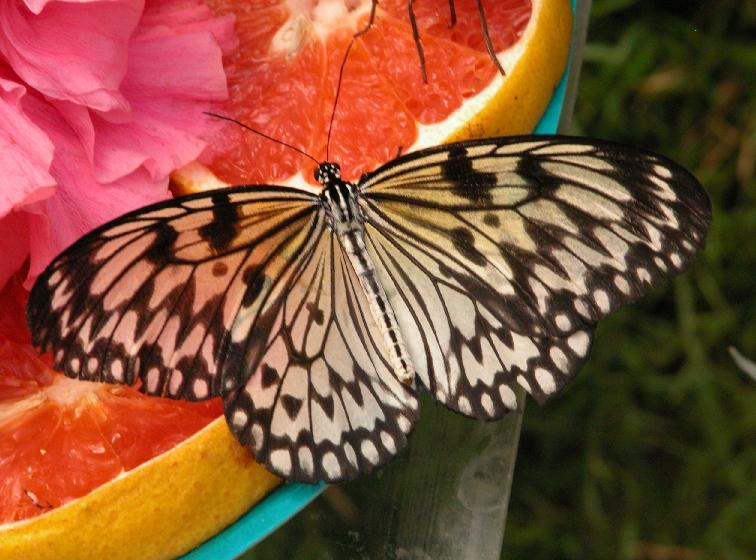
\includegraphics[scale=0.18]{./images/10_puzzles/mcgill_540_7.jpg}}
\\~\\
	Image~(e) \textendash { }540~pieces~\cite{mcgillImageDatabase} & Image~(f) \textendash { }540~pieces~\cite{mcgillImageDatabase}
  \end{tabular}

\caption{First set of six images in the 10~image test set}
\label{fig:firstSet10PuzzleInputImages}
\end{figure}

\begin{figure}
\centering
  \begin{tabular}{ >{\centering\arraybackslash}m{0.47\textwidth} >{\centering\arraybackslash}m{0.47\textwidth} }

	\fbox{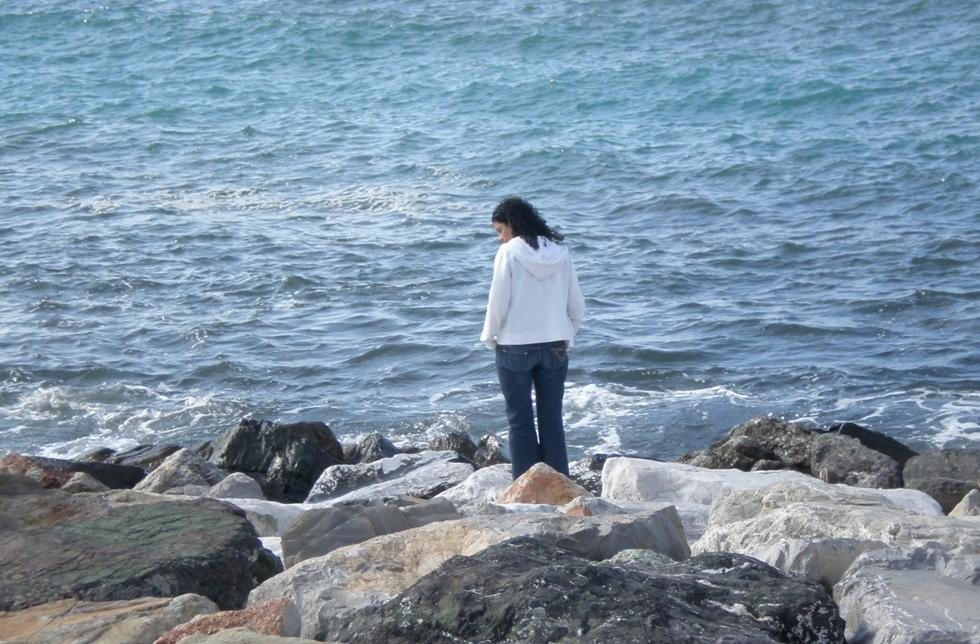
\includegraphics[scale=0.18]{./images/10_puzzles/pomeranz_805_8.jpg}} & \fbox{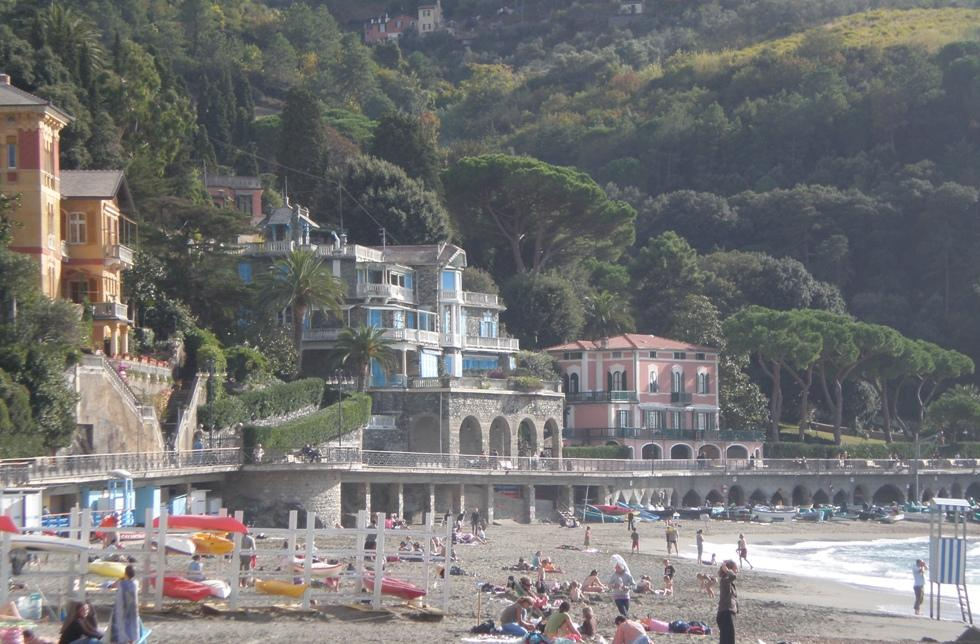
\includegraphics[scale=0.18]{./images/10_puzzles/pomeranz_805_13.jpg}} \\~\\
	Image~(g) \textendash { }805~pieces~\cite{pomeranzBenchmarkImages} & Image~(h) \textendash { }805~pieces~\cite{pomeranzBenchmarkImages} 
\\~\\
	\fbox{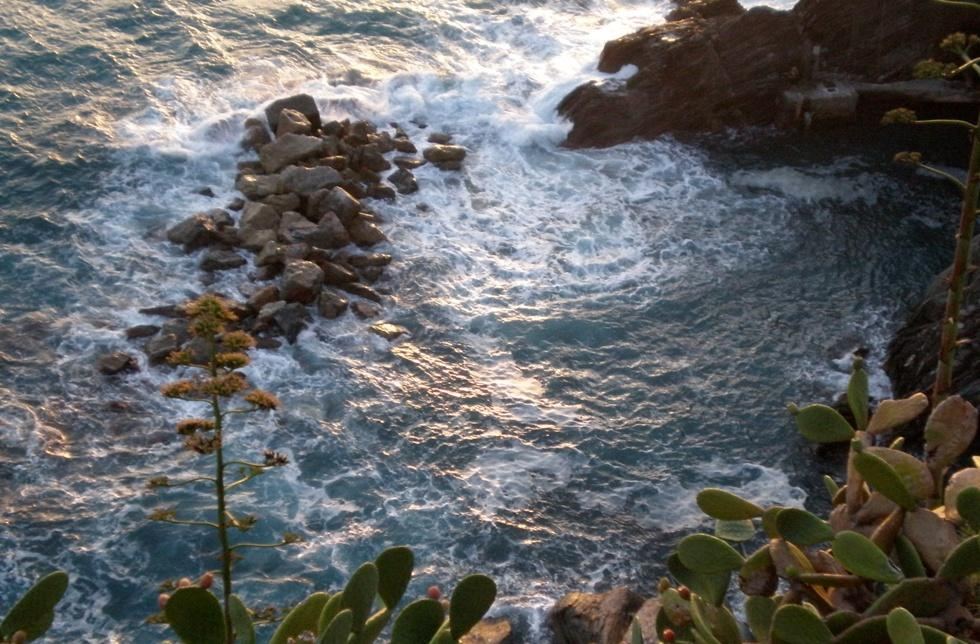
\includegraphics[scale=0.18]{./images/10_puzzles/pomeranz_805_14.jpg}} & \fbox{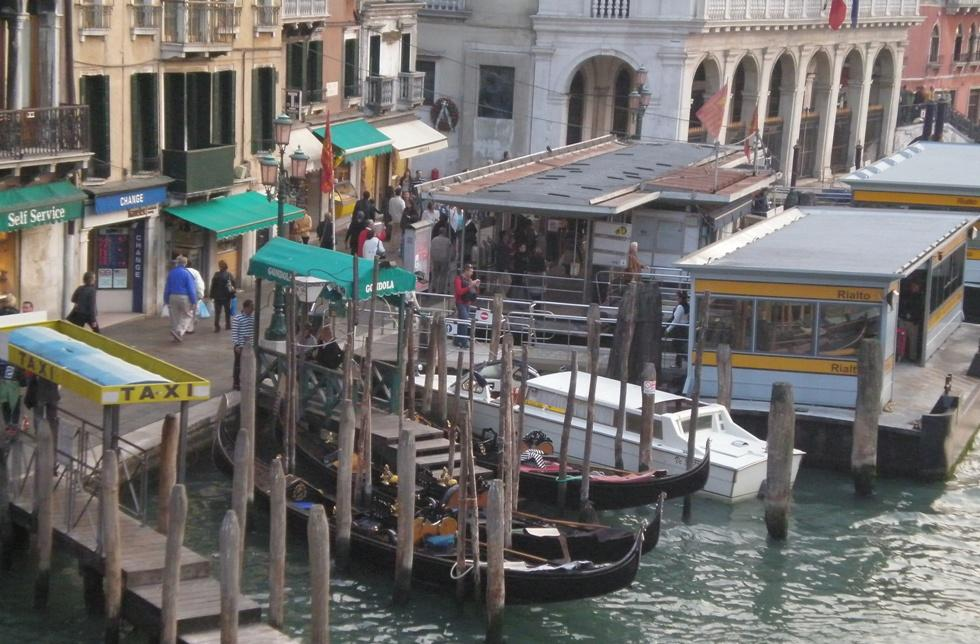
\includegraphics[scale=0.18]{./images/10_puzzles/pomeranz_805_19.jpg}}
\\~\\
	Image~(i) \textendash { }805~pieces~\cite{pomeranzBenchmarkImages} & Image~(j) \textendash { }805~pieces~\cite{pomeranzBenchmarkImages}
  \end{tabular}

\caption{Second set of four images in the 10~image test set. Reproduced with permission from Pomeranz \textit{et. al.}}
\label{fig:secondSet10PuzzleInputImages}
\end{figure}



\begin{figure}
\centering
  \begin{tabular}{ >{\centering\arraybackslash}m{0.47\textwidth} >{\centering\arraybackslash}m{0.47\textwidth} }

	\fbox{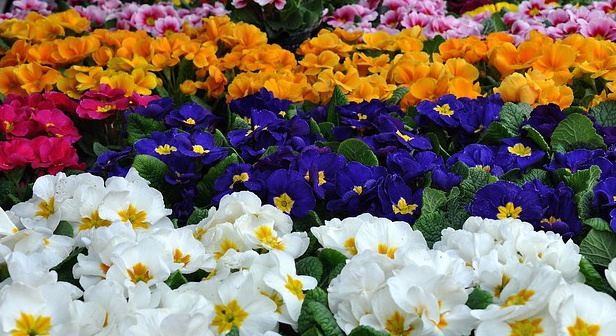
\includegraphics[scale=0.18]{./images/10_puzzles/reconstructed_primula_pixabay.jpg}} & \fbox{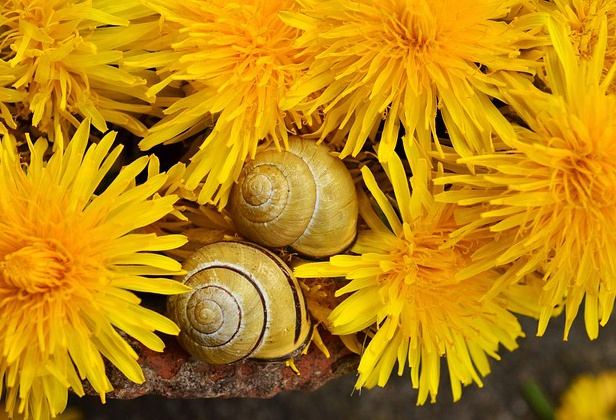
\includegraphics[scale=0.18]{./images/10_puzzles/reconstructed_dandelion_pixabay.jpg}} \\~\\
	Reconstructed image~(a) & Reconstructed image~(b)
\\~\\
	\fbox{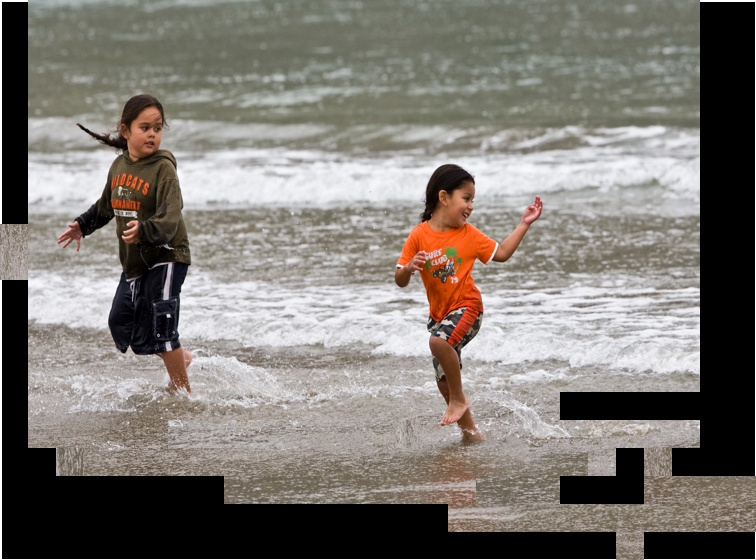
\includegraphics[scale=0.18]{./images/10_puzzles/reconstructed_cho_432_18.jpg}} & \fbox{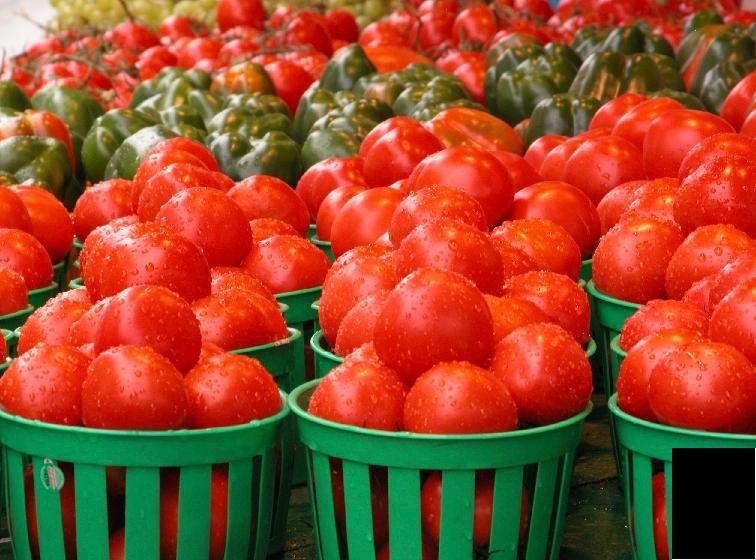
\includegraphics[scale=0.18]{./images/10_puzzles/reconstructed_mcgill_540_16.jpg}} \\~\\
	Reconstructed image~(c) & Reconstructed image~(d) 
\\~\\
	\fbox{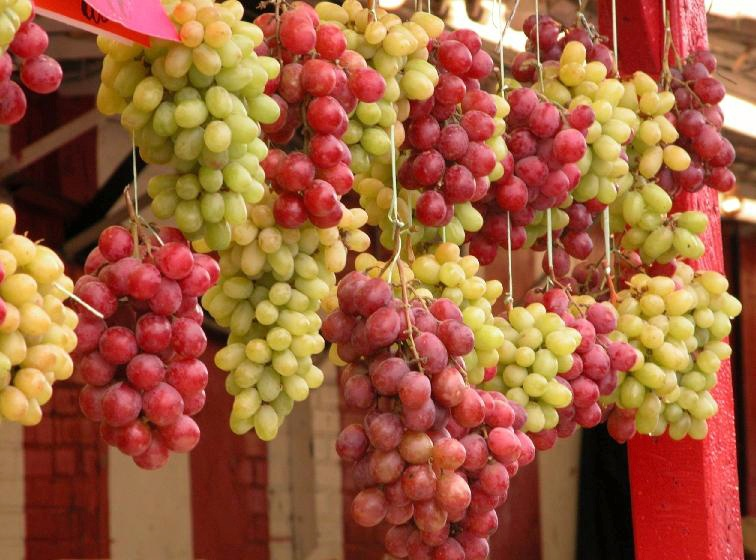
\includegraphics[scale=0.18]{./images/10_puzzles/reconstructed_mcgill_540_15.jpg}} & \fbox{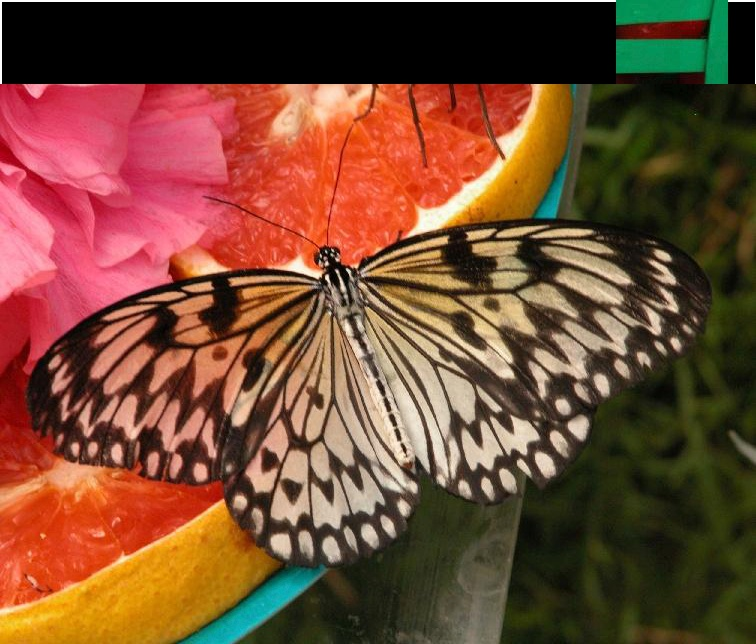
\includegraphics[scale=0.18]{./images/10_puzzles/reconstructed_mcgill_540_7.jpg}}
\\~\\
	Reconstructed image~(e) & Reconstructed image~(f)
  \end{tabular}

\caption{First set of six images output by the Mixed-Bag Solver for the 10~image test set}
\label{fig:firstSet10PuzzleMixedBagSolverImages}
\end{figure}

\begin{figure}
\centering
  \begin{tabular}{ >{\centering\arraybackslash}m{0.47\textwidth} >{\centering\arraybackslash}m{0.47\textwidth} }

	\fbox{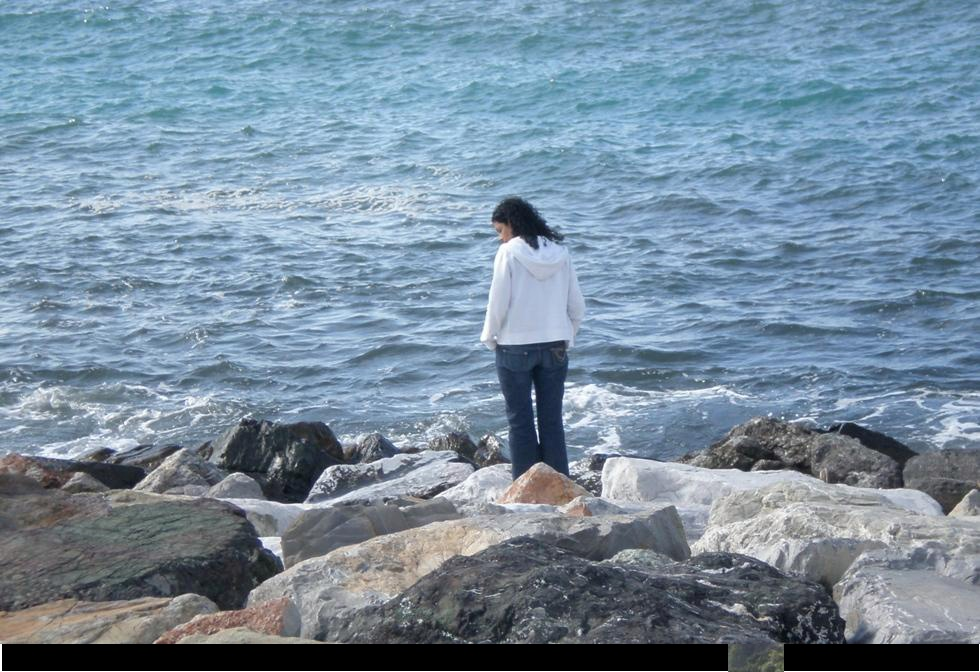
\includegraphics[scale=0.18]{./images/10_puzzles/reconstructed_pomeranz_805_8.jpg}} & \fbox{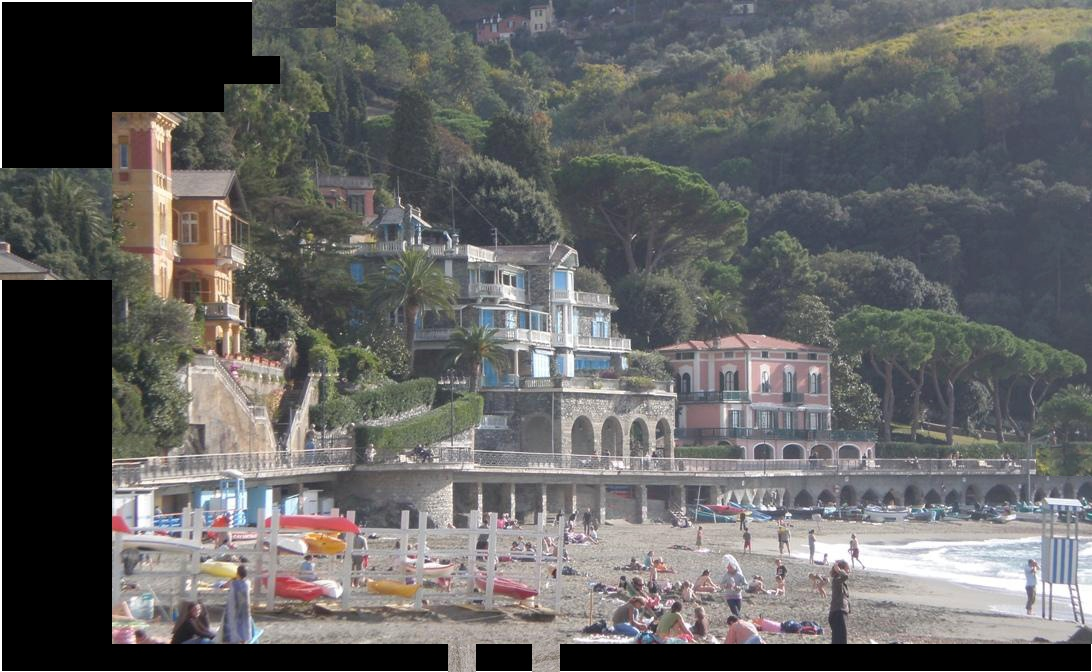
\includegraphics[scale=0.18]{./images/10_puzzles/reconstructed_pomeranz_805_13.jpg}} \\~\\
	Reconstructed image~(g) & Reconstructed image~(h) 
\\~\\
	\fbox{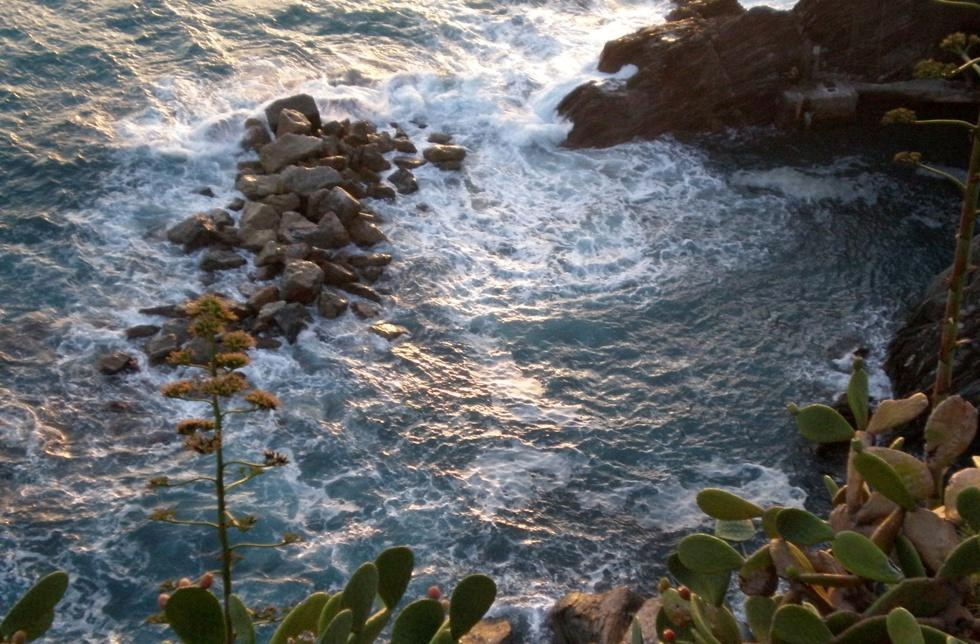
\includegraphics[scale=0.18]{./images/10_puzzles/reconstructed_pomeranz_805_14.jpg}} & \fbox{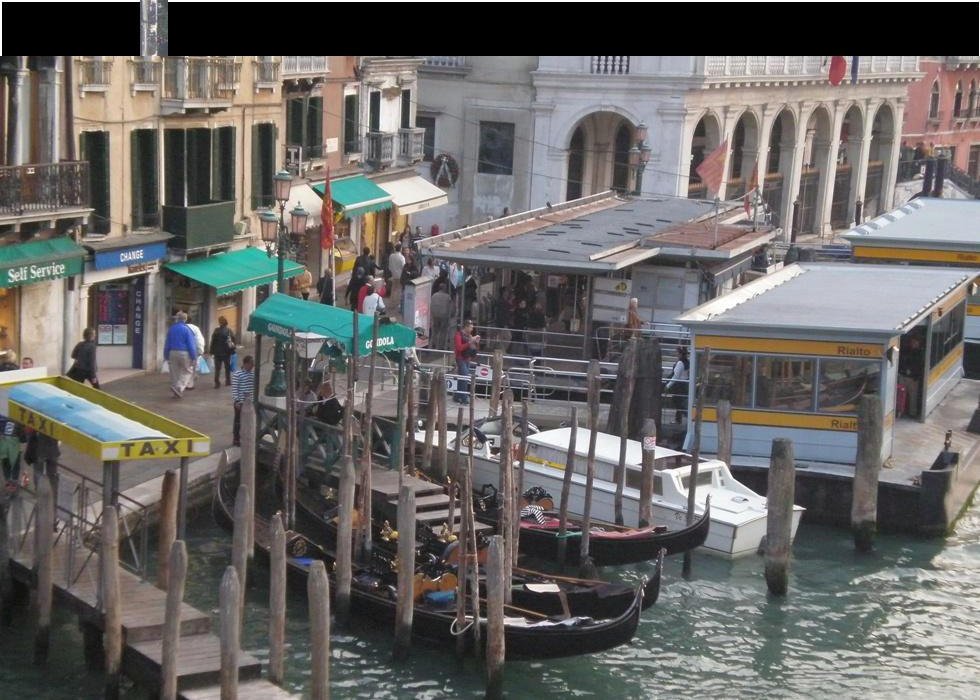
\includegraphics[scale=0.18]{./images/10_puzzles/reconstructed_pomeranz_805_19.jpg}}
\\~\\
	Reconstructed image~(i) & Reconstructed image~(j)
  \end{tabular}

\caption{Second set of four images output by the Mixed-Bag Solver for the 10~image test set}
\label{fig:secondSet10PuzzleMixedBagSolverImages}
\end{figure}


\begin{figure}
\centering
  \begin{tabular}{ >{\centering\arraybackslash}m{0.47\textwidth} >{\centering\arraybackslash}m{0.47\textwidth} }

	\fbox{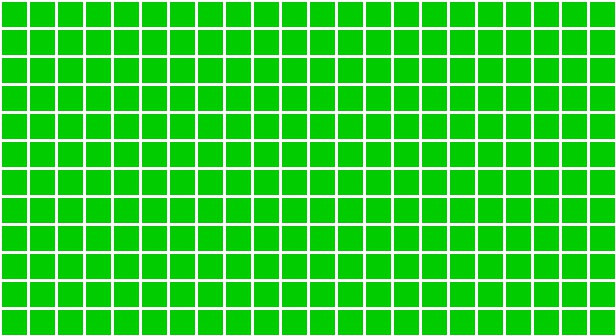
\includegraphics[scale=0.18]{./images/10_puzzles/sedas_primula_pixabay.jpg}} & \fbox{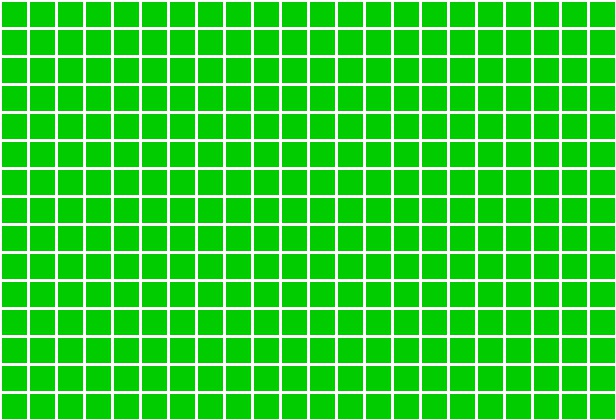
\includegraphics[scale=0.18]{./images/10_puzzles/sedas_dandelion_pixabay.jpg}} \\~\\
	SEDAS visualization of image~(a) & SEDAS visualization of image~(b)
\\~\\
	\fbox{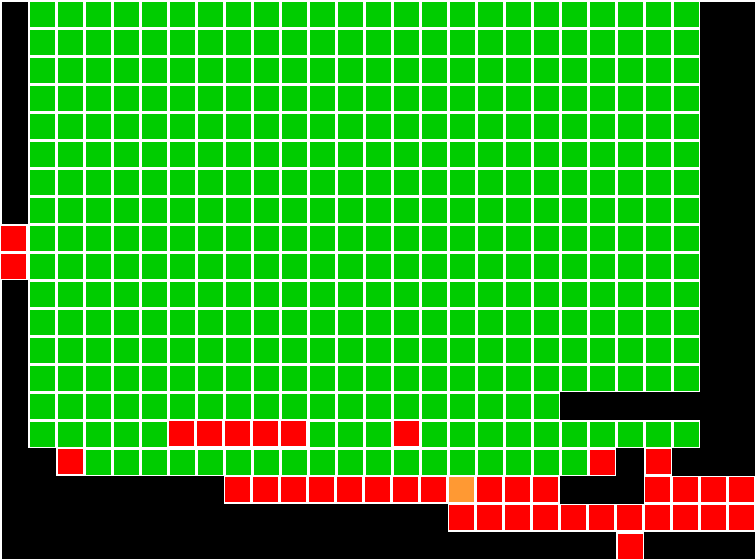
\includegraphics[scale=0.18]{./images/10_puzzles/sedas_cho_432_18.png}} & \fbox{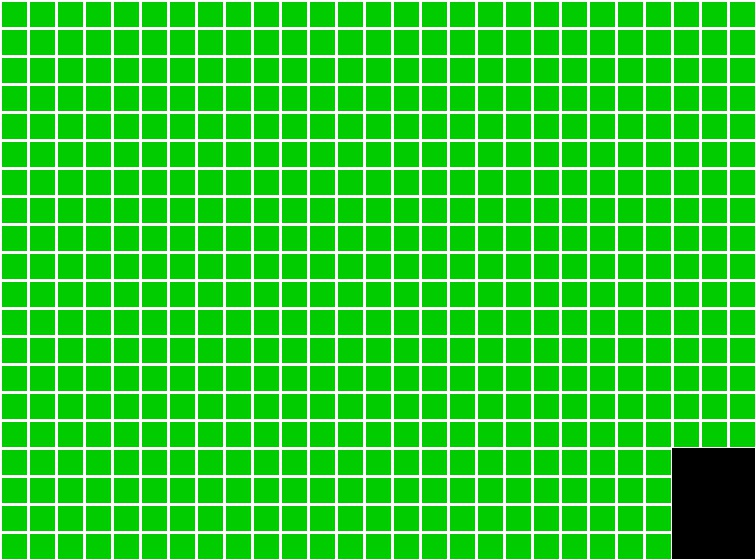
\includegraphics[scale=0.18]{./images/10_puzzles/sedas_mcgill_540_16.jpg}} \\~\\
	SEDAS visualization of image~(c) & SEDAS visualization of image~(d) 
\\~\\
	\fbox{
\includegraphics[scale=0.18]{./images/10_puzzles/sedas_mcgill_540_15.jpg}} & \fbox{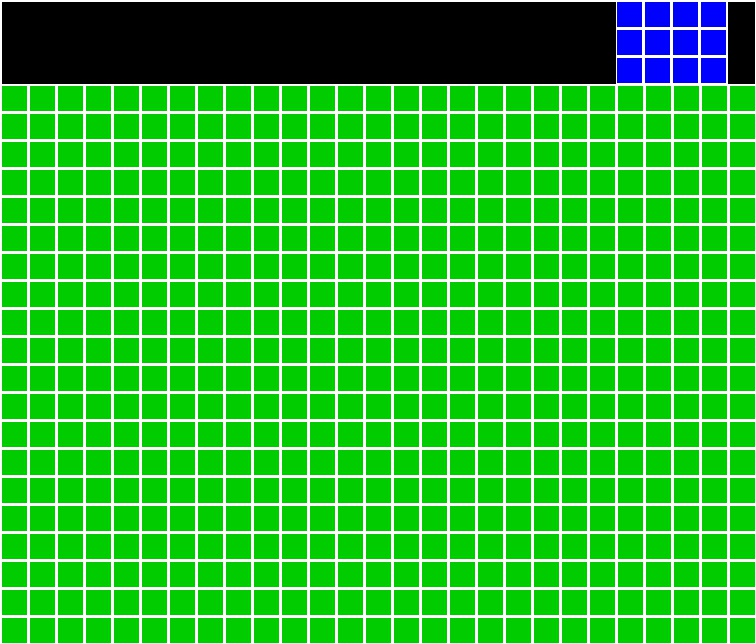
\includegraphics[scale=0.18]{./images/10_puzzles/sedas_mcgill_540_7.jpg}}
\\~\\
	SEDAS visualization of image~(e) & SEDAS visualization of image~(f)
  \end{tabular}

\caption{First set of six SEDAS visualizations for the 10~image test set}
\label{fig:firstSet10PuzzleMixedBagSedasImages}
\end{figure}

\begin{figure}
\centering
  \begin{tabular}{ >{\centering\arraybackslash}m{0.47\textwidth} >{\centering\arraybackslash}m{0.47\textwidth} }

	\fbox{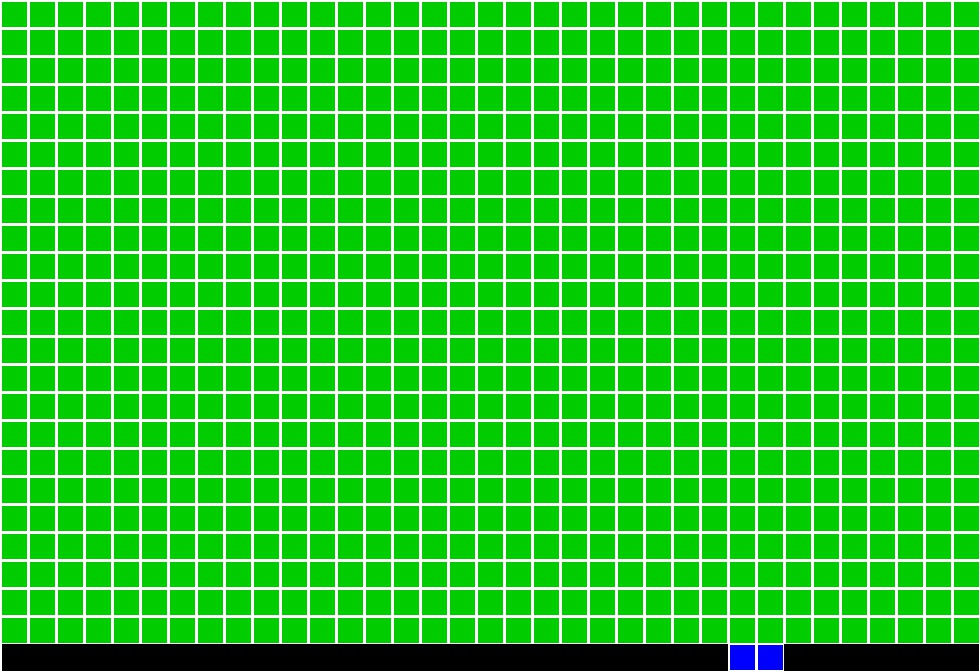
\includegraphics[scale=0.18]{./images/10_puzzles/sedas_pomeranz_805_8.jpg}} & \fbox{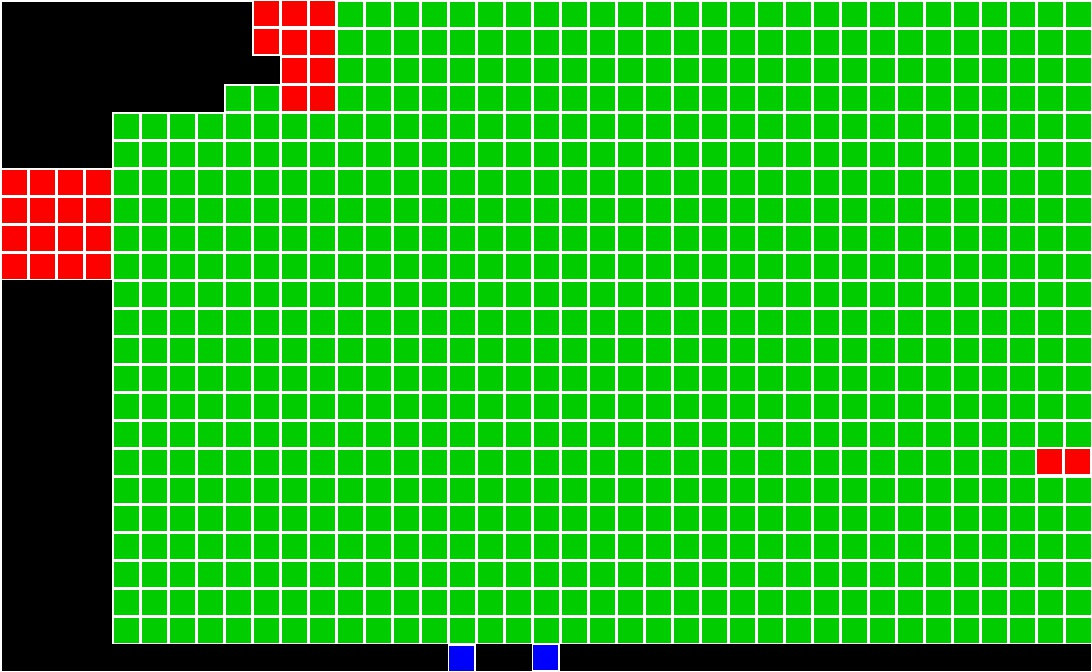
\includegraphics[scale=0.18]{./images/10_puzzles/sedas_pomeranz_805_13.jpg}} \\~\\
	SEDAS visualization of image~(g) & SEDAS visualization of image~(h) 
\\~\\
	\fbox{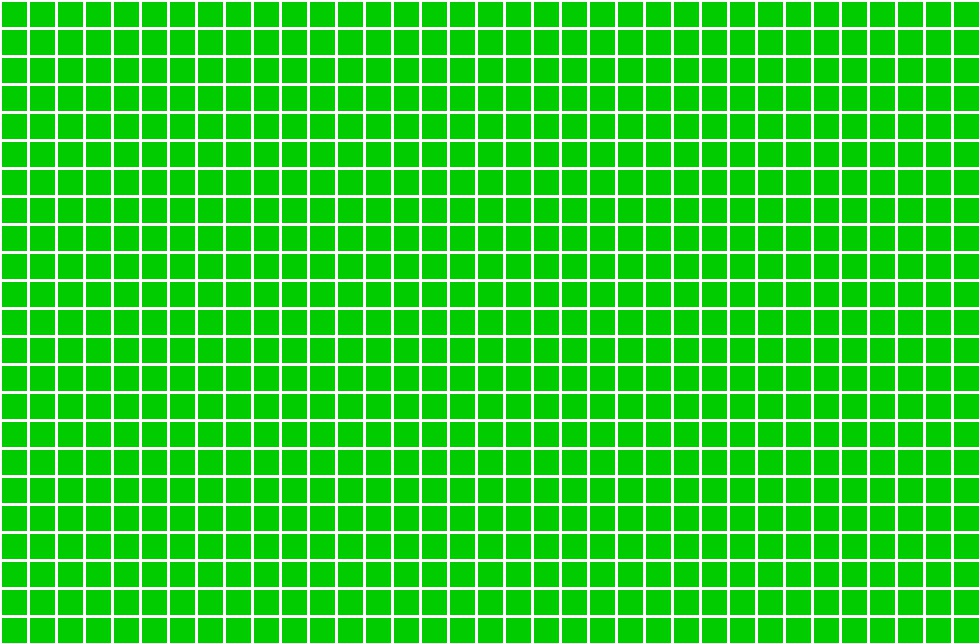
\includegraphics[scale=0.18]{./images/10_puzzles/sedas_pomeranz_805_14.jpg}} & \fbox{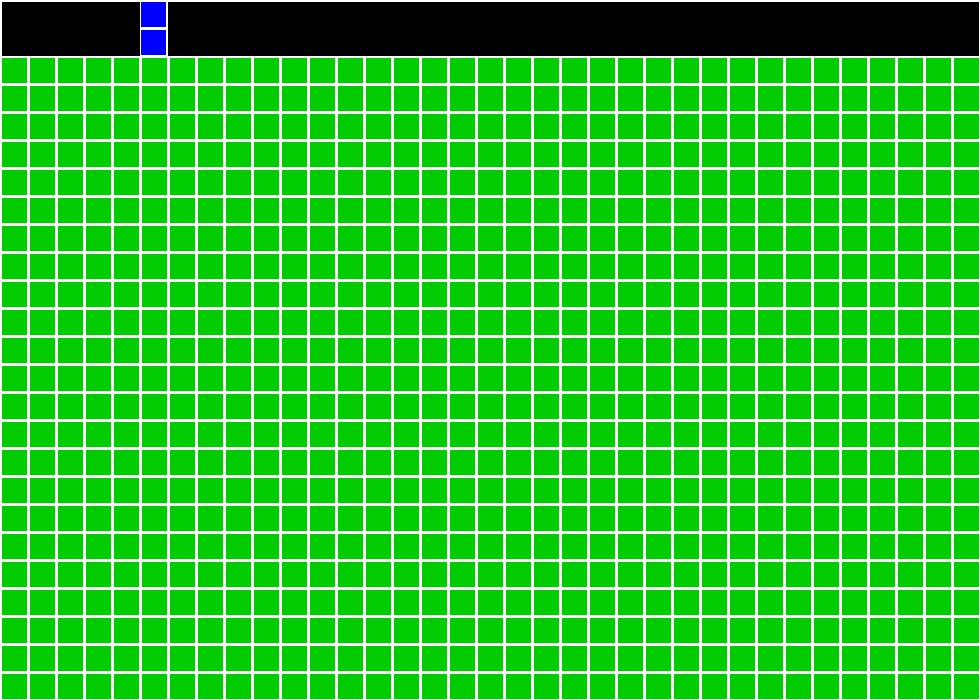
\includegraphics[scale=0.18]{./images/10_puzzles/sedas_pomeranz_805_19.jpg}}
\\~\\
	SEDAS visualization of image~(i) & SEDAS visualization of image~(j)
  \end{tabular}

\caption{Second set of four SEDAS visualizations for the 10~image test set}
\label{fig:secondSet10PuzzleMixedBagSedasImages}
\end{figure}
